\chapter{静电学}
\label{chap:electrostatics}

本章主要为一些基础性内容,分为两节:
\begin{compactenum}
    \item 第一节介绍了静电学(electrostatics)里的一些基本概念、定义等。所谓静,即电荷分布和场均与时间无关(time-independet)。
    \item 第二节主要是一些数学内容,如Green定理、Green函数等。
\end{compactenum}
在历史上,静电学是作为一门研究宏观现象(macroscopic phenomena)的科学而发展起来的,在其中会涉及到一些理想化的概念,如点电荷(point charge)模型。在描述一个点上的电场时,要注意它是宏观上足够小,微观上足够大的一个点。

\section{Coulomb定律}

静电学的全部内容都出于Coulomb定律(Coulomb's law)的定量描述,该实验定律由法国物理学家Charles-Augustin de Coulomb于1785年发表。Coulomb用一系列实验证明:当两个小带电体$q_1,q_2$的距离远大于其本身的线度时,二者在空气中的作用力:
\begin{itemize}
    \item 与每个带电体的电荷量$q_i$成正比;
    \item 与带电体之间距离的平方$\abs{\bm x_1-\bm x_2}$成反比;
    \item 方向沿着这两个电荷的连线;
    \item 如果这两个带电体带异种电荷,则为吸引力;如果带同种电荷,则为排斥力。
\end{itemize}
此外,从实验上还证明了,某一小带电体周围的若干个其他小带电体产生的、作用在该小带电体上的总力,是各两体Coulomb力的矢量和。

\begin{theorem}{Coulomb定律}{Coulomb's law}
    真空中两个静止点电荷$q_1,q_1$分别位于$\bm x_1,\bm x_2$,则$q_1$受到$q_2$的静电力$\bm F_{12}$为:
    \begin{align}
        \label{eqn:Coulomb law}
        \bm F_{12}=k_\elc q_1q_2\frac{\bm x_1-\bm x_2}{|\bm x_1-\bm x_2|^3}.
        % \frac{q_1q_2}{r^2}\uvec r.%
    \end{align}
    % $\bm r:=\bm x_1-\bm x_2$为距离向量,
    其中$k_\elc$是实验测定的系数。SI单位制中
    \[
        k_\elc=\frac1{4\pi\varepsilon_0},
    \]
    其中$\varepsilon_0=\SI{8.8541878128(13)E-12}{C^2/N.m^2}$是真空介电常数(vacuum permittivity)。
\end{theorem}

% Coulomb定律指出:静电力$F\propto 1/r^2$,即。
% 严格地说,Coulomb的结论只适用于真空中的电荷。电介质中的电荷需见\chapref{chap:electrostatics of macroscopic media}中讨论。

\section{电场}

\begin{definition}{电场}{electric field}
    电场(electric field) $\bm E$的强度定义为特定位置的单位电荷所受的力:
    \begin{align}
        \bm E=\frac{\bm F}q.%\bm F=q\bm E,\quad
    \end{align}
    % 在描述一个点上的电场时,要注意它是宏观上足够小、微观上足够大的一个点。
\end{definition}
\begin{remark}
    与定义不同,将带有单位电荷的小带电体放在特定位置所测量得到的力未必是电场强度,因为它的存在可能显著地改变了原场的分布。因此必须采取极限的方法,即测定当小带电体的电荷量越来越小时,作用在其上的力与其电荷量的比值。\footnote{由于电荷是分立的,这种数学极限在物理上不可能实现。这也是宏观电磁学中数学理想化的一个例子。}
\end{remark}

\begin{corollary}
    由Coulomb定律,位于$\bm x_1$的点电荷$q_1$在$\bm x$处激发的电场$\bm E_1$为
    \begin{equation}
        \label{eqn:E of q}
        \bm E_1=kq_1\frac{\bm x-\bm x_1}{|\bm x-\bm x_1|^3};
    \end{equation}
\end{corollary}
\begin{theorem}
    {线性叠加原理}{linear superposition principle}
    实验得知,一系列离散(discrete)点电荷$q_1,\ldots,q_n$在空间中同一点$\bm x$处激发的电场可以线性叠加(linear superposition)
    \begin{equation}
        \label{eqn:E(x) sum}
        \bm E=\sum_{i=1}^n\bm E_i=\frac1{4\pi\varepsilon_0}\sum_{i=1}^nq_i\frac{\bm x-\bm x_i}{|\bm x-\bm x_i|^3},
    \end{equation}
    如果电荷是连续(continuous)分布的,可以用电荷密度$\rho(\bm x)$描述,则求和变成积分:
    \begin{equation}
        \label{eqn:E(x)}
        \bm E(\bm x)=\frac1{4\pi\varepsilon_0}\int_V\rho(\bm x')\frac{\bm x-\bm x'}{|\bm x-\bm x'|^3}\d v'.
    \end{equation}
    式中$\d v'=\d x'\nd y'\nd z'$是在$\bm x'$处的一个三维体积元。
\end{theorem}

\begin{corollary}
    利用Dirac $\delta$函数,电荷密度也可以用来描述分立的点电荷系统:
    \[
        \rho(\bm x')=\sum_{i=1}^nq_i\vd(\bm x'-\bm x_i).
    \]
\end{corollary}

\begin{remark}
    若已知$\rho(\bm x)$,我们可以根据积分\eqref{eqn:E(x)}求解静电场分布,但是这并不总是最适合的方法,下面我们介绍Gauss定律。
\end{remark}

\subsection{Gauss定律}

对于一个点电荷,其场强在一个面$S$上的面积分
\[
    \bm E\cdot\uvec n\d a=\frac q{4\pi\varepsilon_0}\frac{\cos\theta}{r^2}\d a=\frac q{4\pi\varepsilon_0}\d\Omega,
\]
其中$r$是该点电荷到曲面上一点的距离,$\uvec n$是曲面上该点向外的单位法向矢量,$\d a$是面积元,$\theta$是$\bm E$与$\uvec n$的夹角,$\d\Omega$是$\d a$对点电荷所张的立体角(solid angle)元。

因此点电荷场强在一个封闭曲面$\p V$上的面积分为
\[
    \oint_{\p V}\bm E\cdot\uvec n\d a=\begin{cases}
        q/\varepsilon_0,&q~\text{在}~V~\text{内}\\
        0,&q~\text{在}~V~\text{外}
    \end{cases}
\]
由此便得到了静电场的Gauss定律:
\begin{theorem}{Gauss定律}{Gauss's law}
    对于分立的点电荷系,电场$\bm E$在一个封闭曲面$\p V$上的面积分为$V$内的所有电荷求和:
    \begin{equation}
        \oint_{\p V}\bm E\cdot\uvec n\d a=\frac1{\varepsilon_0}\sum_{V}q_i,
    \end{equation}
    对于电荷密度为$\rho(\bm x)$的连续分布电荷来说,
    \begin{equation}
        \label{eqn:Gauss law}
        \oint_{\p V}\bm E\cdot\uvec n\d a=\frac1{\varepsilon_0}\int_V\rho(\bm x)\d v,
    \end{equation}
\end{theorem}

\begin{corollary}
    根据推导过程,Gauss定律依赖于:
    \begin{itemize}
        \item 电荷间作用力满足平方反比定律;
        \item 作用力是有心力;
        \item 不同电荷效应可以线性叠加。
    \end{itemize}
    因此,对于Newton引力场来说,Gauss定律也成立。
\end{corollary}

\begin{remark}
    尽管Gauss定律总是对的,但并不总是有用。只有在满足一些对称性条件时,电场的面积分才比较容易求。%比如对于均匀带电的球(或球壳)外部激发的电场与同电荷在球心的点电荷相同。
\end{remark}

\begin{example}{无限大平板的静电场}{E of infinite plate}
    无限大平板带有均匀面电荷密度$\sigma$,%求其电场。
    由对称性,空间中任意一点处的电场一定是垂直平面向外的,
    对一个截面为$A$的横跨平面的Gauss小药盒(pillbox)使用Gauss定律
    \[
        2EA=\frac{\sigma A}{\varepsilon_0}\implies\bm E=\frac\sigma{2\varepsilon_0}\uvec n.
    \]
    $\uvec n$为指向远离平面的单位法向量。
    \begin{center}
        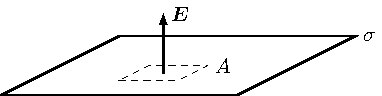
\includegraphics[page=1]{figures/tikz/layouts.pdf}
        \captionof{figure}{无限大平板的静电场}
        \label{fig:infinite plate}
    \end{center}
\end{example}
\begin{example}{无限长直线}{E of infinite line}
    无限长直线有均匀线电荷密度$\lambda$,由对称性,电场是垂直直线向外的,对一个高$H$半径$\rho$的同轴圆柱使用Gauss定律
    \[
        E\cdot 2\pi\rho H=\frac{\lambda H}{\varepsilon_0}\implies\bm E=\frac{\lambda}{2\pi\varepsilon_0\rho}\uvec\rho.
    \]
    \begin{center}
        \includegraphics[page=2]{figures/tikz/layouts.pdf}
        \captionof{figure}{无限长直线的静电场}
        \label{fig:infinite line}
    \end{center}
    \tcblower
    可以证明,均匀带电半圆在圆心处的电场与距离为半径的无限长直线的电场相同,因为可以构造二者微元的一一映射,如\figref{fig:semicircle <=> line} 所示。
    \begin{center}
        \includegraphics[page=3]{figures/tikz/layouts.pdf}
        \captionof{figure}{半圆与直线微元的一一映射}
        \label{fig:semicircle <=> line}
    \end{center}
\end{example}

\paragraph{Gauss定律的微分形式}

由散度定理\eqref{eqn:div},
\[
    \oint_{\p V}\bm A\cdot\uvec n\d a=\int_V\div\bm A\d v
\]
结合Gauss定律\eqref{eqn:Gauss law},可得
\[
    \int_V\biggkh{\div\bm E-\frac\rho{\varepsilon_0}}\d v\equiv 0
\]
该式对任意$V$均成立。由此被积分式为零。
\begin{theorem}{Gauss定律的微分形式}{differential form of Gauss's law}
    \begin{equation}
        \label{eqn:divE}
        \div\bm E=\frac\rho{\varepsilon_0}.
    \end{equation}
\end{theorem}

\section{标量势}

由恒等式\footnote{在同时存在多个变量时,约定:$\nabla$不带下标时,默认作用在$\bm x$上;特别地,当作用在$\bm x'$上时,$\nabla_{\bm x'}$可简记为$\nabla'$。}
\[
    \nabla\biggkh{\frac1{|\bm x-\bm x'|}}=-\frac{\bm x-\bm x'}{|\bm x-\bm x'|^3}.
\]
可将电场\eqref{eqn:E(x)}写成梯度的形式:
\[
    \bm E(\bm x)=-\frac1{4\pi\varepsilon_0}\nabla\biggkh{\int_V\frac{\rho(\bm x')}{|\bm x'-\bm x|}\d v'}
\]
\begin{definition}{标量势}{scalar potential}
    定义标量势(或电势、电位,potential)满足
    \begin{align}
        \label{eqn:gradPhi}
        \bm E=-\nabla\Phi.
    \end{align}
    显然满足上式的$\Phi$并不唯一,但它们之间仅相差一个常量,因此在讨论电位时我们需要提前选定某一参考点(通常是无穷远处)电位为0。$\Phi$的最简单的形式是:
    \begin{align}
        \label{eqn:Phi-rho}
        \Phi(\bm x):=\frac1{4\pi\varepsilon_0}\int_V\frac{\rho(\bm x')}{|\bm x'-\bm x|}\d v'.
    \end{align}
\end{definition}

\begin{corollary}
    在电场$\bm E$下将试探电荷$q$从$A$点移动到$B$点时,克服电场力而对电荷所做的功
    \[
        W=-\int_A^Bq\bm E\cdot\d\bm\ell=q(\Phi_B-\Phi_A).
    \]
    上式表明$q\Phi$可解释为试探电荷在电场中的势能。
\end{corollary}

\paragraph{静电场的旋度}

由\eqref{eqn:curlgrad}梯度的旋度为0,可得除Gauss定律\eqref{eqn:Gauss law}外的另一个微分方程:
\begin{theorem}{静电场无旋}{curlless E}
    \begin{equation}
        \label{eqn:curlE}
        \curl\bm E=\bm 0.
    \end{equation}
\end{theorem}
这也可从任意闭合路径的电场线积分为0得到。

\paragraph{导体}
导体(conductor)是易于传导电荷的物质,其内部存在大量%可以自由移动的
自由电荷(free charge)。因此稳定时,导体内部不会存在静电场或静电电荷(因为自由电荷会在静电场下快速移动到导体表面达到平衡态),并且导体表面和内部都是等势的。
\begin{example}{带电导体球的电势}{potential of conducting sphere}

    半径为$R$的均匀导体球携带电荷$q$,%易得这些电荷均匀地分布在导体球表面,
    由Gauss定律,电场分布
    \[
        \bm E(r)=
        \begin{cases}
            \bm 0,&r<R\\
            \frac1{4\pi\varepsilon_0}\frac q{r^2}\uvec r,&r>R
        \end{cases}
    \]
    参考点设置为无穷远处,则电势
    \[
        \Phi(r)=-\int_{+\infty}^r\bm E\cdot\d\bm r=
        \begin{cases}
            \frac1{4\pi\varepsilon_0}\frac qR,&r<R\\
            \frac1{4\pi\varepsilon_0}\frac qr,&r>R
        \end{cases}.
    \]
    \begin{center}
        \includegraphics[page=4]{figures/tikz/layouts.pdf}
        \captionof{figure}{带电导体球的电势}
        \label{fig:conducting sphere}
    \end{center}
\end{example}

\section{电荷的表面分布}

考察面电荷密度为$\sigma$的表面,表面法向单位矢量$\uvec n$从表面的一侧(1)指向另一侧(2),根据Gauss定律,电场法向分量在表面两侧是不连续的:
\begin{equation}
    \label{eqn:En2-En1}
    (\bm E_2-\bm E_1)\cdot\uvec n=\frac\sigma{\varepsilon_0}.
\end{equation}
而电场切向分量是连续的:
\begin{equation}
    (\bm E_2-\bm E_1)\times\uvec n=\bm 0.
\end{equation}

再来看电位在表面上的分布,式\eqref{eqn:En2-En1}可以写成:
\begin{equation}
    -\pv{\Phi_2}{\uvec n}+\pv{\Phi_1}{\uvec n}=\frac\sigma{\varepsilon_0}.
\end{equation}
可以证明,在体电荷和面电荷分布上,电位分布是连续的。但是对于点电荷、线电荷或电偶层(dipole layers),电位分布是不连续的!
\begin{example}{电偶层}{dipole layers}
    两个面电荷密度为$\sigma$、间距为$d$的电偶层的电位 
    \begin{align*}
        \Phi(\bm x)=\frac1{4\pi\varepsilon_0}\int_S\frac{\sigma(\bm x')}{|\bm x-\bm x'|}\d a'-\frac1{4\pi\varepsilon_0}\int_{S'}\frac{\sigma(\bm x')}{|\bm x-\bm x'+d\uvec n|}\d a''
    \end{align*}
    由三维Taylor展开,
    \[
        \frac1{|\bm x+\bm a|}=\frac1x+\bm a\cdot\nabla\biggkh{\frac1x}+\cdots,\quad a\ll x.
    \]
    可得当$d\to0$时,
    %\frac1{|\bm x-\bm x'+d\uvec n|}\simeq\frac1{|\bm x-\bm x'|}+d\uvec n\cdot\nabla_{\bm x-\bm x'}\biggkh{\frac1{|\bm x-\bm x'|}}
    \[
        \Phi(\bm x)\simeq-\frac1{4\pi\varepsilon_0}\int_S\sigma(\bm x')d\uvec n\cdot\biggfkh{-\nabla'\biggkh{\frac1{|\bm x-\bm x'|}}}\d a'
    \]
    其中
    \[
        \uvec n\cdot\nabla'\biggkh{\frac1{|\bm x-\bm x'|}}\d a'=-\frac{\cos\theta}{|\bm x-\bm x'|^2}\d a'=-\d\Omega.
    \]
    定义层矩(surface-dipole-moment density) 
    \[
        D(\bm x):=\lim_{d\to 0}d(\bm x)\sigma(\bm x)
    \]
    则
    \begin{equation}
        \Phi(\bm x)=-\frac1{4\pi\varepsilon_0}\int_SD(\bm x')\d\Omega.
    \end{equation}
    电位在电偶层两边会发生跳变
    \begin{equation}
        \Phi_2-\Phi_1=\frac D{\varepsilon_0}.
    \end{equation}
\end{example}

\section{电场的能量}

取无穷远点为参考点,一系列点电荷$q_1,\ldots,q_n$所带的静电势能(electrostatic potential energy)可通过归纳法得出:
\begin{align}
    W=\frac1{4\pi\varepsilon_0}\sum_{i=1}^n\sum_{j=1}^{i-1}\frac{q_iq_j}{|\bm x_i-\bm x_j|}=\frac1{8\pi\varepsilon_0}\sum_{i\neq j}\frac{q_iq_j}{|\bm x_i-\bm x_j|}.
\end{align}
对于连续分布的电荷:
\begin{align*}
    \label{eqn:W-qq}
    W=\frac1{8\pi\varepsilon_0}\iint_V\frac{\rho(\bm x)\rho(\bm x')}{|\bm x-\bm x'|}\d v\nd v'.
\end{align*}
注意上式没有要求$\bm x\neq\bm x'$,可代入式\eqref{eqn:Phi-rho},
\begin{align}
    W=\frac12\int_V\rho(\bm x)\Phi(\bm x)\d v.
\end{align}
可对上式进行变形,由式\eqref{eqn:divE}和\eqref{eqn:gradPhi},$\rho=\varepsilon_0\div\bm E=-\varepsilon_0\lapla\Phi$,
\begin{align*}
    W=-\frac{\varepsilon_0}2\int_V\Phi\lapla\Phi\d v=-\frac{\varepsilon_0}2\biggfkh{\oint_{\p V}\Phi\nabla\Phi\cdot\d\bm a-\int_V|\nabla\Phi|^2\d v}
\end{align*}
%由分部积分,\int_Vf\div\bm A\d v=\oint_{\p V}f\bm A\cdot\d\bm a-\int_V\bm A\cdot\nabla f\d v
%取$f=\Phi,\enspace\bm A=\nabla\Phi$,
由于$V$是整个空间,故边界(无穷远处)的$\Phi=0$,
因此我们用场的形式表示静电势能
\begin{align}
    \label{eqn:W-E}
    W=\frac{\varepsilon_0}2\int_V|\bm E|^2\d v
\end{align}
并可定义能量密度(energy density)
\begin{align}
    w=\frac{\varepsilon_0}2|\bm E|^2.
\end{align}

% 现在我们来审视式\eqref{eqn:W-qq}和式\eqref{eqn:W-E},
观察表达式,式\eqref{eqn:W-E}当然恒为正,但式\eqref{eqn:W-qq}却不一定。一种解释认为:式\eqref{eqn:W-qq}仅包含了互能(电荷间相互作用的静电势能),而式\eqref{eqn:W-E}包含了互能和自能(构成点电荷自身所需要的能量)。
\begin{example}{导体的能量密度}{energy density of conductor}
    由式\eqref{eqn:Et2-Et1},导体内的电场$\bm E_\text{in}=\bm 0$,故导体的法向电场
    \[
        \bm E=\frac\sigma{\varepsilon_0}\uvec n,\quad w=\frac{\varepsilon_0}2|\bm E|^2=\frac{\sigma^2}{2\varepsilon_0}.
    \]
\end{example}

\paragraph{导体系统、电容}
考虑一系列导体构成的系统,导体所带电荷分别为$Q_1,\ldots,Q_n$,由线性关系,导体表面电势
\[
    V_i=\sum_{j=1}^np_{ij}Q_j,
\]
$p_{ij}$取决于导体的几何关系,这相当于一个矩阵,取逆即
\begin{align}
    Q_i=\sum_{j=1}^nC_{ij}V_j.
\end{align}
\begin{compactitem}
	\item $C_{ii}$即导体的电容(capacitance),其物理意义是:当导体保持在单位电位、所有其他导体都保持在零电位时的导体的总电荷;
	\item $C_{ij}$是感应系数(coefficients of induction),%可以用来
    表示两个导体系统的电容。
\end{compactitem}
导体系统的势能
\[
    W=\frac12\sum_{i=1}^nQ_iV_i=\frac12\sum_{i=1}^n\sum_{j=1}^nC_{ij}V_iV_j.
\]

\section{数学内容}

\begin{definition}
    {Poisson方程和Laplace方程}{}
    结合式\eqref{eqn:divE}和\eqref{eqn:gradPhi},便会得到Poisson方程
    \begin{align}
        \label{eqn:Poisson}
        \lapla\Phi=-\frac\rho{\varepsilon_0}.
    \end{align}
    特别地,$\rho\equiv 0$时,变成Laplace方程
    \begin{align}
        \label{eqn:Laplace}
        \lapla\Phi=0.
    \end{align}
\end{definition}
%式\eqref{eqn:Phi-rho}可以是Poisson方程的一个解。
求解电势$\Phi$分布就需要求解Poisson方程\eqref{eqn:Poisson},但是只有$V$内的条件是不够的,边界$\p V$上的电位也会影响$V$内的电场和电势分布。

\subsection{Green定理}

散度定理\eqref{eqn:div}
\[
    \int_V\div\bm A\d v=\oint_{\p V}\bm A\cdot\uvec n\d a
\]
取$\bm A:=\phi\nabla\psi$,
% 则左右两边的积分项分别为
% \begin{align*}
%     \div(\phi\nabla\psi)&=\nabla\phi\cdot\nabla\psi+\phi\lapla\psi,\\
%     \phi\nabla\psi\cdot\uvec n&=\phi\pv\psi n.
% \end{align*}
便得到了第一Green公式:

\begin{theorem}{Green定理}{Green's theorem}
    第一Green公式
    \begin{equation}
        \label{eqn:Green 1}
        \int_V(\nabla\phi\cdot\nabla\psi+\phi\lapla\psi)\d v=\oint_{\p V}\phi\pv\psi n\d a.
    \end{equation}
    将$\phi,\psi$轮换后两式相减,得到第二Green公式
    \begin{equation}
        \label{eqn:Green 2}
        \int_V(\phi\lapla\psi-\psi\lapla\phi)\d v=\oint_{\p V}\biggkh{\phi\pv\psi n-\psi\pv\phi n}\d a.
    \end{equation}
\end{theorem}

利用第二Green公式\eqref{eqn:Green 2},我们令$\phi:=\Phi(\bm x'),\enspace\psi:=|\bm x-\bm x'|^{-1}$,则
\[
    \nabla'^2\phi=-\frac{\rho}{\varepsilon_0},\quad\nabla'^2\psi=-4\pi\vd(\bm x-\bm x'),
\]
我们选定$\bm x\in V$使得$\delta$函数的积分项得以保留,代入并移项得到
%\int_V\biggfkh{-4\pi\Phi(\bm x')\vd(\bm x-\bm x')+\frac{\rho}{\varepsilon_0R}}\d v'=\oint_{\p V}\biggfkh{\Phi\pp{n'}\biggkh{\frac1R}-\frac1R\pv\Phi{n'}}\d a'
%4\pi\Phi(\bm x)+\frac1{\varepsilon_0}\int_V\frac{\rho}{R}\d v'=\oint_{\p V}\biggfkh{\Phi\pp{n'}\biggkh{\frac1R}-\frac1R\pv\Phi{n'}}\d a'
\begin{equation}
    \label{eqn:Phi-rho with boundary}
        \Phi(\bm x)=\frac1{4\pi\varepsilon_0}\int_V\frac{\rho(\bm x')}{|\bm x-\bm x'|}\d v'+\frac1{4\pi}\oint_{\p V}\biggfkh{\frac1{|\bm x-\bm x'|}\pv\Phi{n'}-\Phi(\bm x')\pp{n'}\biggkh{\frac1{|\bm x-\bm x'|}}}\d a',
\end{equation}
与式\eqref{eqn:Phi-rho}对比,上式多了两项边界$\p V$上的积分,分别等价于面电荷的电势($\p\Phi/\p n'$不连续)
\[
    \begin{cases}
        \Phi(\bm x)=\frac1{4\pi\varepsilon_0}\oint_{\p V}\frac{\sigma(\bm x')}{|\bm x-\bm x'|}\d a'\\[2ex]
        \sigma(\bm x')=\varepsilon_0\pv\Phi{n'}.
    \end{cases}
\]
和电偶层的电势($\Phi$不连续)
\[
    \begin{cases}
        \Phi(\bm x)=\frac1{4\pi\varepsilon_0}\oint_{\p V}D(\bm x')\pp{n'}\biggkh{\frac1{|\bm x-\bm x'|}}\d a'\\
        D(\bm x')=-\varepsilon_0\Phi(\bm x').
    \end{cases}
\]
因此,求解$V$内的电势$\Phi$分布问题,除了需要$V$内电荷密度$\rho$的分布,还需知道表面$\p V$上的电势条件($\Phi$或$\p\Phi/\p n$),这称为边界条件(boundary condition)。
我们可以对不同的边界条件进行分类:
\begin{definition}{边界条件}{boundary condition}
    Dirichlet边界条件:给定表面上的电位
    \[
        \Phi|_{\p V}=f;
    \]
    Neumann边界条件:给定表面上电位的法向导数
    \[
        \edg{\pv\Phi n}_{\p V}=f;
    \]
    混合边界条件
\end{definition}

\subsection{唯一性定理}

\begin{theorem}{唯一性定理}{uniqueness theorem}
    给定封闭体积$V$及边界$\p V$上的Dirichlet (或Neumann)边界条件,得到Poisson方程的解是唯一的。
\end{theorem}
\begin{proof}
    若存在两个解$\Phi_1,\Phi_2$满足同一个边界条件。令$U:=\Phi_1-\Phi_2$,则
\[
    \begin{cases}
        \nabla^2U=0,\\
        U|_{\p V}=0\enspace\text{或}\enspace\edg{\pv Un}_{\p V}=0,
    \end{cases}
\]
由Green第一公式\eqref{eqn:Green 1},令式中$\phi=\psi=U$,则
\[
    \int_V(U\lapla U+\nabla U\cdot\nabla U)\d v=\oint_{\p V}U\pv Un\d a,
\]
即
\[
    \int_V|\nabla U|^2\d v=0\implies|\nabla U|\equiv 0\implies U=\const.
\]
这说明$\Phi_1$和$\Phi_2$仅相差一个常数。对电位来说,这仅是参考点的差别。%唯一性定理得证。
\end{proof}
%对于Dirichlet边界条件,直接$U\equiv 0$,故解是唯一的;对于Neumann边界条件,

\subsection{Green函数法求解Poisson方程}
\label{ssec:Green solve Poisson}

由于式\eqref{eqn:Phi-rho with boundary}同时出现了$\Phi$和$\p\Phi/\p n$的边界条件,因此它并不适合解静电场方程。我们需要寻找一种只含Dirichlet或Neumann边界条件的解。下面我们引入Green函数。
\begin{definition}{Green函数}{Green function}
    Green函数是满足如下方程的一系列函数:
    \begin{align}
        \nabla'^2G(\bm x,\bm x')=-4\pi\vd(\bm x-\bm x').
    \end{align}
\end{definition}
回到第二Green公式\eqref{eqn:Green 2},这次令$\phi:=\Phi(\bm x'),\enspace\psi:=G(\bm x,\bm x')$,式\eqref{eqn:Phi-rho with boundary}变为
\begin{align*}
    \Phi(\bm x)=\frac1{4\pi\varepsilon_0}\int_V\rho(\bm x')G(\bm x,\bm x')\d v'+\frac1{4\pi}\oint_{\p V}\biggfkh{G(\bm x,\bm x')\pv\Phi{n'}-\Phi(\bm x')\pv G{n'}}\d a'.
\end{align*}

\paragraph{对于Dirichlet边界条件}我们可设法找到一个$G$满足:
\begin{equation}
    \label{eqn:Dirichlet Green condition}
    G(\bm x,\bm x')|_{\p V}\equiv 0,\tag{$\ast$}
\end{equation}
上式变为:
\begin{align}
    \label{eqn:Dirichlet Green}
    \Phi(\bm x)=\frac1{4\pi\varepsilon_0}\int_V\rho(\bm x')G(\bm x,\bm x')\d v'-\frac1{4\pi}\oint_{\p V}\Phi(\bm x')\pv G{n'}\d a';
\end{align}

\paragraph{对于Neumann边界条件}由
\[
    \oint_{\p V}\pv G{n'}\d a'=\int_V\nabla'^2G(\bm x,\bm x')\d v=-4\pi,
\]
我们也可以设法找到一个$G$满足:
\begin{equation}
    \label{eqn:Neumann Green condition}
    \edg{\pv G{n'}}_{\p V}\equiv-\frac{4\pi}S,\tag{$\ast\ast$}
\end{equation}
则
\begin{align}
    \label{eqn:Neumann Green}
    \Phi(\bm x)=\ave\Phi_{\p V}+\frac1{4\pi\varepsilon_0}\int_V\rho(\bm x')G(\bm x,\bm x')\d v'+\frac1{4\pi}\oint_{\p V}G(\bm x,\bm x')\pv\Phi{n'}\d a',
\end{align}
其中$\ave\Phi_{\p V}$是边界上的平均电势
\[
    \ave\Phi_{\p V}:=\frac1S\oint_{\p V}\Phi(\bm x')\d a'.
\]
上述方法不依赖于边界条件的具体形式,因此是普遍的。但通常很难找到一个满足\eqref{eqn:Dirichlet Green condition}或\eqref{eqn:Neumann Green condition}的$G(\bm x, \bm x')$,因为它依赖于$\p V$的形状。
\begin{example}{Green函数举例}{}
    在无边界空间$V=\RR^3$中,可取
    \[
        G(\bm x,\bm x')=\frac1{|\bm x-\bm x'|}=\frac1{\sqrt{(x-x')^2+(y-y')^2+(z-z')^2}}.
    \]
    在上半空间$V=\set{(x,y,z)}{z>0}$中,为了运用式\eqref{eqn:Dirichlet Green},需要$G$在$\p V=\{(x,y,0)\}$处为0。可取$\bm x'$的对称点$\bm x''=(x',y',-z')$,并取
    \begin{align*}
        G(\bm x,\bm x')&=\frac1{|\bm x-\bm x'|}-\frac1{|\bm x-\bm x''|}\\
        &=\frac1{\sqrt{(x-x')^2+(y-y')^2+(z-z')^2}}-\frac1{\sqrt{(x-x')^2+(y-y')^2+(z+z')^2}}.
    \end{align*}
\end{example}
\begin{theorem}
    {Green函数的对称性}{}
    对于Dirichlet边界条件,Green函数是对称的:
    \[
        G(\bm x,\bm x')=G(\bm x',\bm x);
    \]
    但对于Neumann边界条件,还需加上一项才是对称的:
    \[
        G(\bm x,\bm x')+\frac1S\oint_{\p V}G(\bm x,\bm x'')\d a''=G(\bm x',\bm x)+\frac1S\oint_{\p V}G(\bm x',\bm x'')\d a'',
    \]
    额外加的这一项并不影响电势$\Phi(\bm x)$。
\end{theorem}
Green函数可被拆解为
\[
    G(\bm x,\bm x')=\frac1{|\bm x-\bm x'|}+F(\bm x,\bm x'),
\]
而$F$满足$V$内的Laplace方程
\[
    \nabla'^2F(\bm x,\bm x')=0.
\]
$F(\bm x, \bm x')$与电像法有关(后面会讨论)。
其物理意义为:
$F(\bm x, \bm x')/4\pi\varepsilon_0$表示$V$外的电荷系统的势。

\subsectionstar{变分法}

泛函(functional)是指从函数空间到实数(或复数)的映射,并被认为是一个函数的函数。泛函通常表示为包含函数及其导数的定积分。
\begin{align}
    I\bigfkh{y(x)}=\int_a^bf\bigkh{x,y(x),y'(x)}\d x
\end{align}
\begin{definition}{变分原理}{variational principle}
    在变分微积分中使用的一种科学原理,它发展了寻找函数的一般方法,这些函数使依赖于这些函数的量的值极值。

    比如:最小作用量原理、物理学中的Hamilton原理、静电学中的Thomson定理、光学中的Fermat原理
\end{definition}
Dirichlet边界条件的泛函
\[
    I(\psi)=\frac12\int_V\nabla\psi\cdot\nabla\psi\d v-\int_Vg\psi\d v
\]

\subsectionstar{松弛法}

松弛法是一种迭代的数值格式(有时称为迭代有限差分法)。
\[
    \frac{\D f}{\D x}=\frac{f(x+h)-f(x)}h
\]

